\end{tabular}
\ifsidenote
\begin{tikzpicture}[overlay,remember picture]
\path[<-,line width=2pt] ($(sidenote) + (2,0.2)$) edge[bend right] ++(1.5,1);
\node [align=center] at ($(sidenote) + (3.5,2)$) {<notice>:\\\textit{<side-msg>}};
\end{tikzpicture}
\fi
\raggedright

\vspace{1em} \hspace{2em}
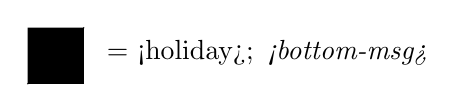
\begin{tikzpicture}[scale=.7]
\draw[\oddcolor, fill=\oddcolor] (0,0) -- (1,0) -- (1,1) -- cycle;
\draw[\evencolor, fill=\evencolor] (0,0) -- (0,1) -- (1,1) -- cycle;
\node [right] at (1.25,0.55) {= <holiday>;\enskip\textit{<bottom-msg>}};
\end{tikzpicture}
\hspace{2em}
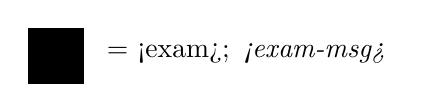
\begin{tikzpicture}[scale=.7]
\draw[\examcolor, fill=\examcolor] (0,0) -- (1,0) -- (1,1) -- (0,1);
\node [right] at (1.25,0.55) {= <exam>;\enskip\textit{<exam-msg>}};
\end{tikzpicture}

\end{document}
